\onehalfspacing
We demonstrate the success of the GA on synthetically simulated ideal and noisy fault-slip observations, and an example of published fault-slip observations from Tymbaki, Greece (Angelier, 1979).

\section{Synthetic Fault-Slip Observations}
Given a reduced stress tensor, we compute the direction and sense of shear stress/slip on a fault plane. We have randomly sampled the strike and dip values for simulations. These values follow a uniform probability density function. Only those striated fault planes are used that obey the Byerlee’s law (1978), i.e., the ratio of the shear to the normal stress $\ge$ 0.85. Using known values of the reduced stress tensors, synthetic fault-slip observations are simulated for extensional, compressional, strike-slip and oblique tectonic settings (Fig. 6A-D). The first three tectonic settings are defined by vertically directed $\sigma_{1}$, $\sigma_{2}$ and $\sigma_{3}$ respectively, whereas none of the principal stresses are vertical in the oblique tectonic setting. Each set of synthetically simulated fault-slip observations is analysed by the GA and the results are compared with true values in the known stress tensors. In all the four tectonic settings, the results given by the GA are consistent with the true values in respective reduced stress tensors (Table 1).

We have also used the synthetic fault-slip observations for comparison of the GA with other common methods, the 4-D exploration (Angelier, 1984) and the direct inversion (Angelier, 1990). These methods also produce acceptable results in situations where one of the principal stresses is vertical (Table 1). However, in the oblique tectonic settings, where none of principal stresses are vertical, these methods may give results that deviate significantly from the true values (Table 1). This may be attributed to the possibility that the inversion becomes highly nonlinear when the axes are inclined and the direct methods get trapped in a locally optimum solution. Similarly, in the existing implementations of the 4-D exploration, a starting point of the algorithm is predefined using the inversion results from the direct inversion, hence the results tend to be similar. A detailed analysis of all the methods are required to further comment upon this deviation, which is beyond the scope of this study.

\section{Noisy Fault-Slip Observations}
Data sets obtained from the fault-slip observations in field are commonly noisy. To test the effect of noise on the GA, we added eight percent random noise, following the uniform distribution, to the each of the synthetic observations strike, dip and rake in oblique tectonic setting (Fig. 6D) and obtained the noisy data set (Fig. 6E). For noisy data, the GA produces results that have deviation commensurate with noise added to data (Table 1). This choice of noise percentage is arbitrary and as the noise percentage increases, so will the deviation from the true value.

\section{Natural Fault-Slip Observations}
We have tested the validity of the GA on many natural fault-slip observations. Here, we present a typical test on a natural example of fault-slip observations from Tymbaki, Greece (Angelier, 1979, 1990). This example has been commonly used for testing the validity of different methods (Michael, 1984; Hardcastle and Hills, 1991; Yin and Ranalli, 1995). The results from GA compare well with those given by the direct inversion and the 4-D exploration (Fig 6F, Table 2). It is noteworthy that the principal stress orientations are close to Andersonian orientation in this example.

\pagebreak
%\begin{landscape}
\begin{table}[H]
  \footnotesize
  \centering
  \renewcommand{\arraystretch}{1.5}
  \begin{tabular}{@{}ccccccccc@{}}
    \toprule
    \multicolumn{4}{c}{True values (Given stress tensor)} & Method & Ratio & \multicolumn{3}{c}{Principal stress orientation} \\
    
    \midrule
    
    $\phi$ & $\sigma_1$ & $\sigma_2$ & $\sigma_3$ & & $\phi$ & $\sigma_1$ & $\sigma_2$ & $\sigma_3$ \\
    
    \cmidrule(lr){1-4} \cmidrule(lr){6-9}
  
    0.20 & 000/90 & 090/00 & 000/00 & 4D & 0.21 & 011/89 & 269/00 & 179/01 \\
    
    \multicolumn{4}{c}{Extensional Setting (Fig. 6A)} & DI & 0.20 & 152/90 & 270/00 & 000/00 \\
    
    \multicolumn{4}{c}{ } & GA & 0.21 & 000/90 & 090/00 & 000/00 \\
    \midrule
    
    0.90 & 180/00 & 090/00 & 000/90 & 4D & 1.00 & 224/00 & 314/00 & 077/90 \\
    
    \multicolumn{4}{c}{ Compressional Setting (Fig. 6B)} & DI & 0.90 & 357/00 & 087/00 & 226/90 \\
     
    \multicolumn{4}{c}{ } & GA & 0.89 & 180/00 & 090/00 & 000/90 \\
    \midrule
    
    0.40 & 180/00 & 000/90 & 270/00 & 4D & 0.40 & 179/03 & 356/87 & 089/00 \\
    
    \multicolumn{4}{c}{ Strike-slip Setting (Fig. 6C)} & DI & 0.43 & 180/01 & 338/89 & 090/00 \\
     
    \multicolumn{4}{c}{ } & GA & 0.41 & 180/00 & 270/89 & 270/01 \\
    \midrule

     0.50 & 134/50 & 334/38 & 236/10 & 4D & 0.61 & 319/66 & 146/24 & 055/03 \\
    
    \multicolumn{4}{c}{ Oblique Setting (Fig. 6D)} & DI & 0.49 & 320/72 & 148/18 & 057/02 \\
     
    \multicolumn{4}{c}{ } & GA & 0.44 & 137/52 & 332/37 & 237/07 \\
    \midrule

     0.50 & 134/50 & 334/38 & 236/10 & 4D & 0.76 & 318/78 & 163/22 & 072/05 \\
    
    \multicolumn{4}{c}{ Noisy Data (Fig. 6E)} & DI & 0.65 & 332/78 & 165/11 & 075/03 \\
     
    \multicolumn{4}{c}{ } & GA & 0.33 & 150/55 & 342/34 & 249/06 \\
    \midrule
    \multicolumn{9}{l}{\textit{Note}:4D- 4D exploration, DI- Direct Inversion, GA- Genetic Algorithm.}
    \bottomrule
  \end{tabular}
  \caption{Test of GA on synthetic examples and comparison with other methods.}\label{table:1}
\end{table}

\begin{table}[H]
  \footnotesize
  \centering
  %\renewcommand{\arraystretch}{1.5}
  \begin{tabular}{@{}ccccc@{}}
    \toprule
    Method & Ratio & \multicolumn{3}{c}{Principal stress orientations}\\
    \cmidrule(lr){2-5} \\
     &  $\phi$ & $\sigma_1$ & $\sigma_2$ & $\sigma_3$ \\
    \midrule
    
    4D & 0.07 & 275/82 & 057/06 & 147/05 \\
    DI & 0.05 & 186/85 & 065/03 & 335/04 \\
    GA & 0.06 & 100/79 & 044/06 & 315/09 \\
    
    \midrule
    \multicolumn{5}{l}{\textit{Note}: Abbreviations same as Table 1.}
    \bottomrule
  \end{tabular}
  \caption{Application of GA on a natural example and its comparison with other methods.}\label{table:2}
\end{table}

\begin{figure}[H]
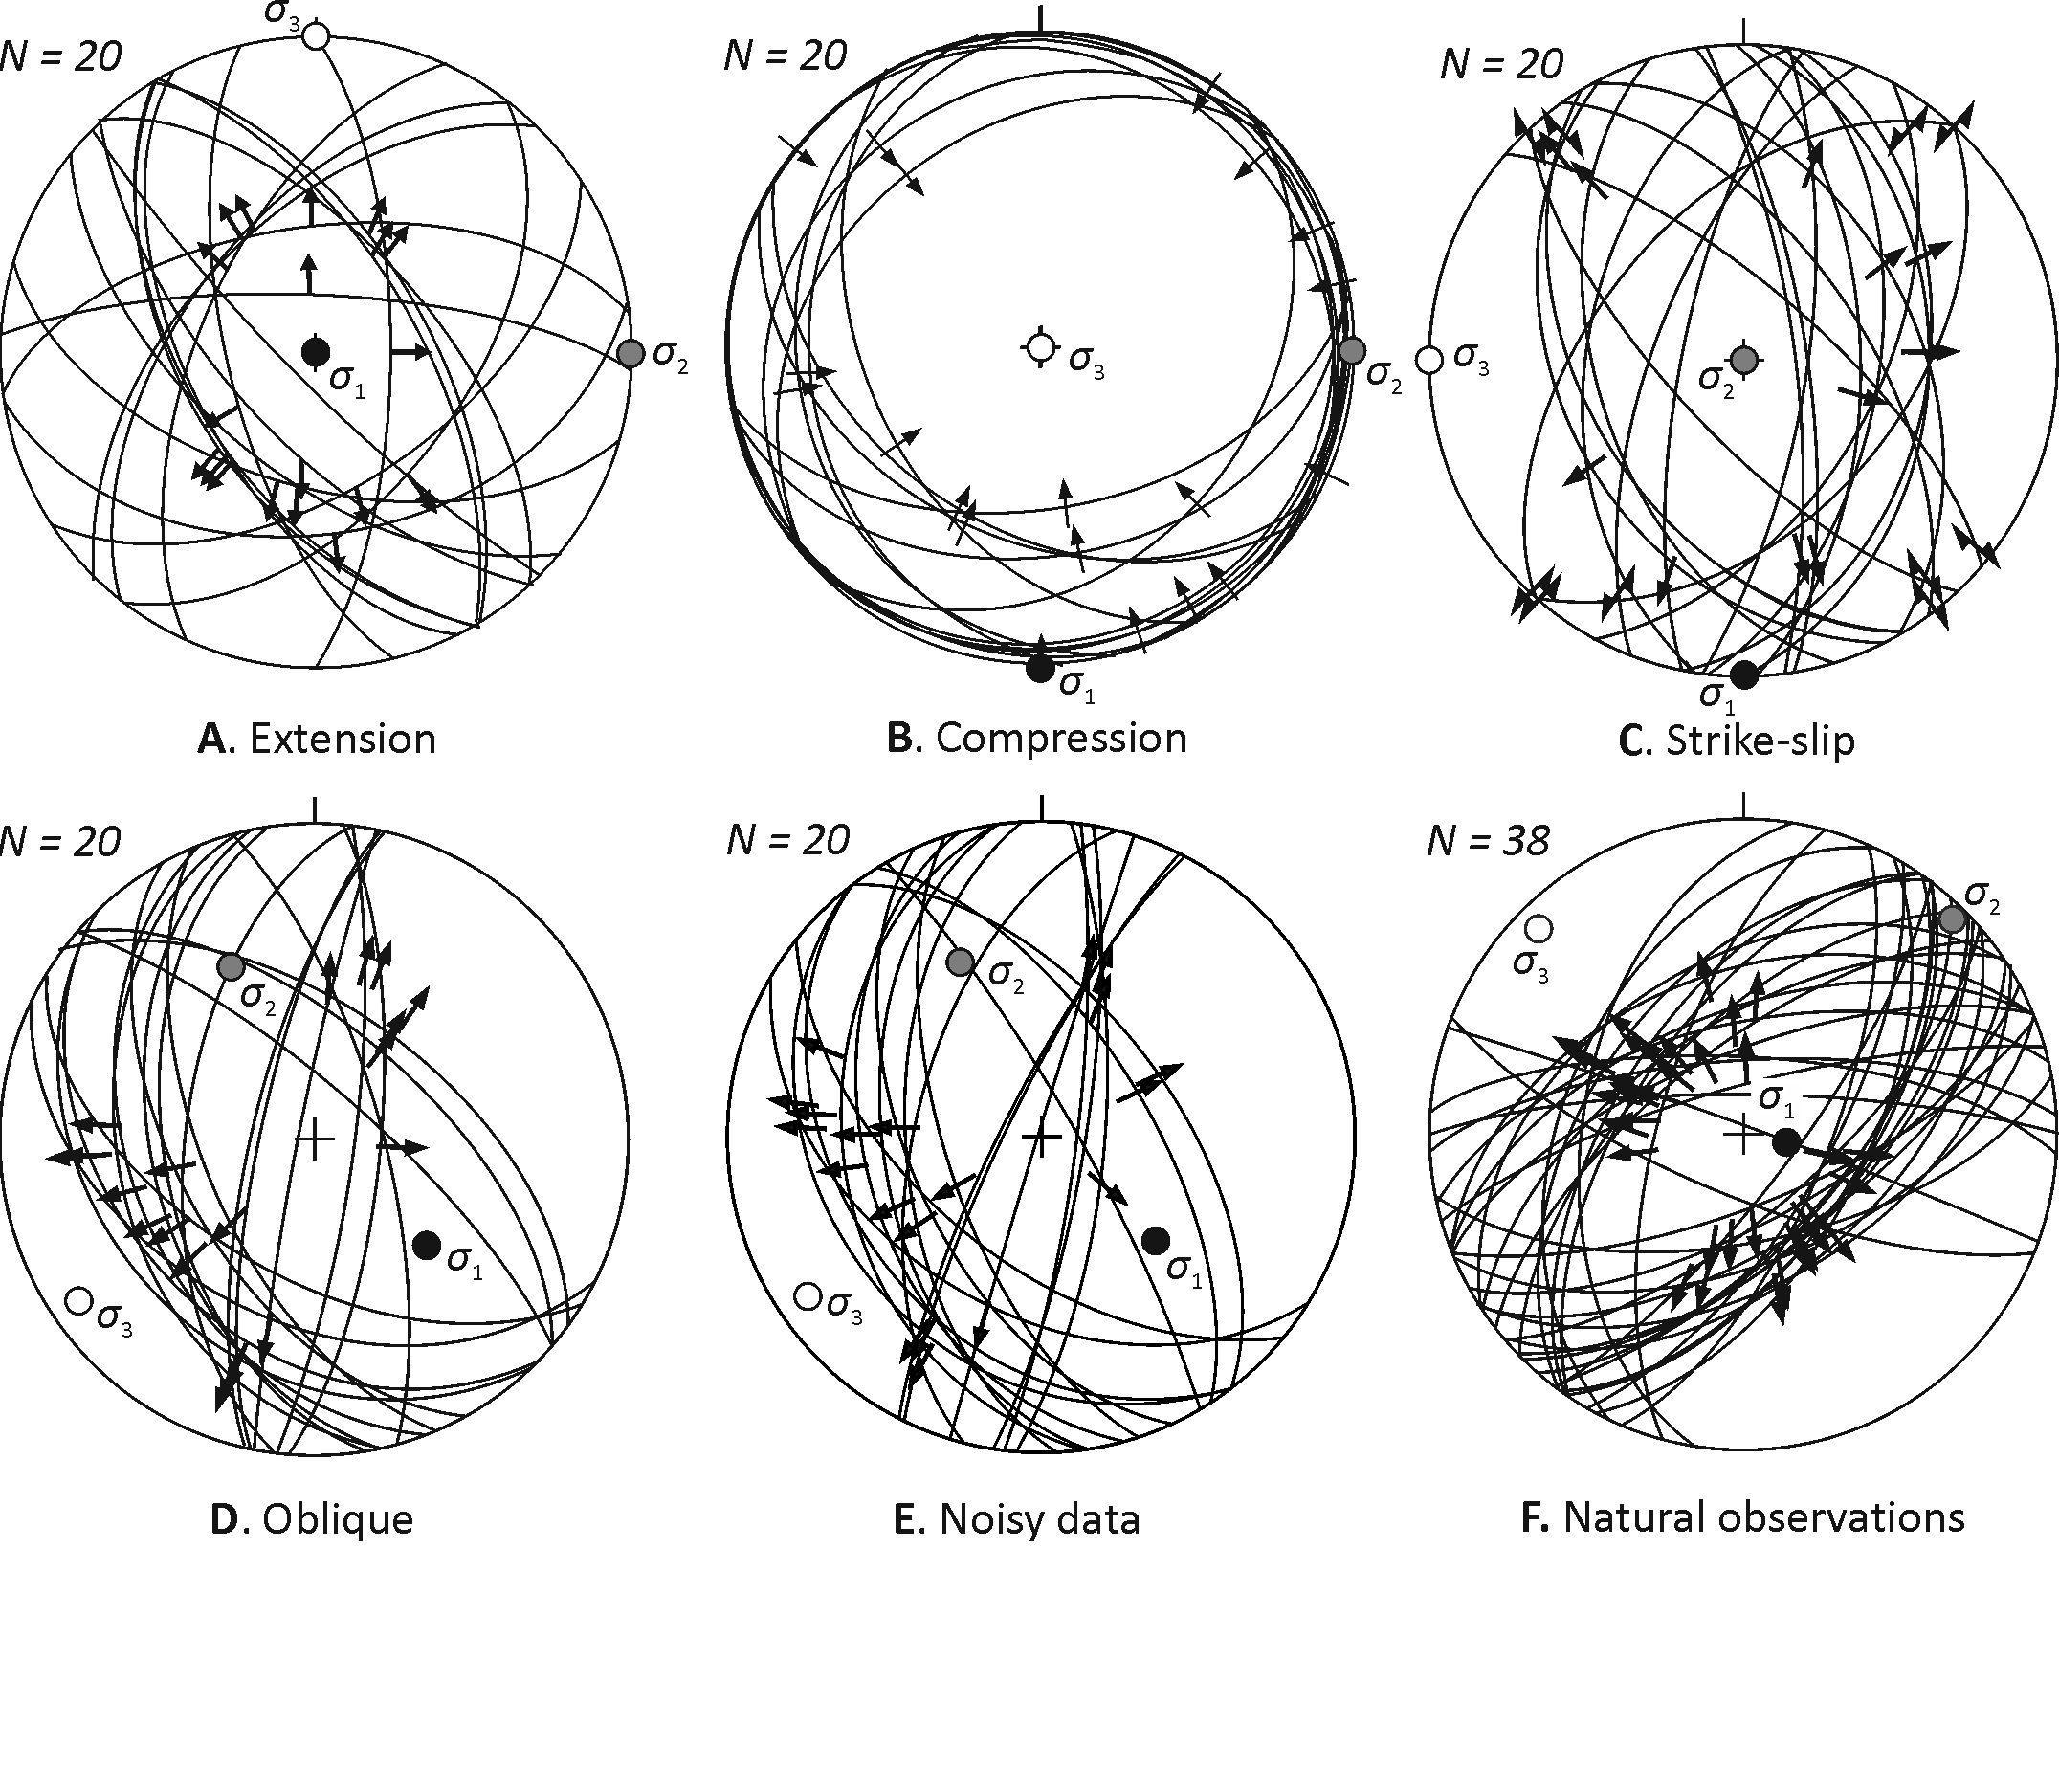
\includegraphics[scale=0.24]{Fig6}
\caption{Validation of the GA. \textbf{A-E}: Synthetic fault-slip observations in four different tectonic settings. \textbf{A}: Extensional, \textbf{B}: Compressional, \textbf{C}: Strike-slip, \textbf{D}: Oblique tectonic setting. \textbf{E}: Noisy data set. \textbf{F}: Natural fault-slip observations (Angelier, 1979).}
\label{fig6}
\end{figure}